\begin{frame}{Conclusions}

  \begin{itemize}
    \item ElGamal permutations behave like random for cycle sizes and distribution of graph
    \item ElGamal permutations are close to random permutations for nonlinearity
    \item ElGamal sequences have balance and periodicity close to random
    \item Tuples in ElGamal sequences are distributed as in random balanced sequences
    \item Run lengths in ElGamal sequences satisfy Golomb's Randomness Postulate
    \end{itemize}
  
\end{frame}

\begin{frame}{Next steps}

  \begin{itemize}
  \item Experiments indicate that $\lambda(z)$ bounds are tight.  So any improvements will be conditional
  \item Prove properties of the distribution of $\lambda(z)$
  \item Prove linear complexity results for ElGamal sequences
  \item Determine expected linear complexity for random balanced random sequences
  \item Further investigate auto-correlation
    \item Will these be enough to justify cryptographic utility? 
    \end{itemize}
  
\end{frame}


\begin{frame}{}

  \begin{center}
  \scalebox{3}{Obrigado} \\

  \scalebox{3}{Thanks} \\

  
  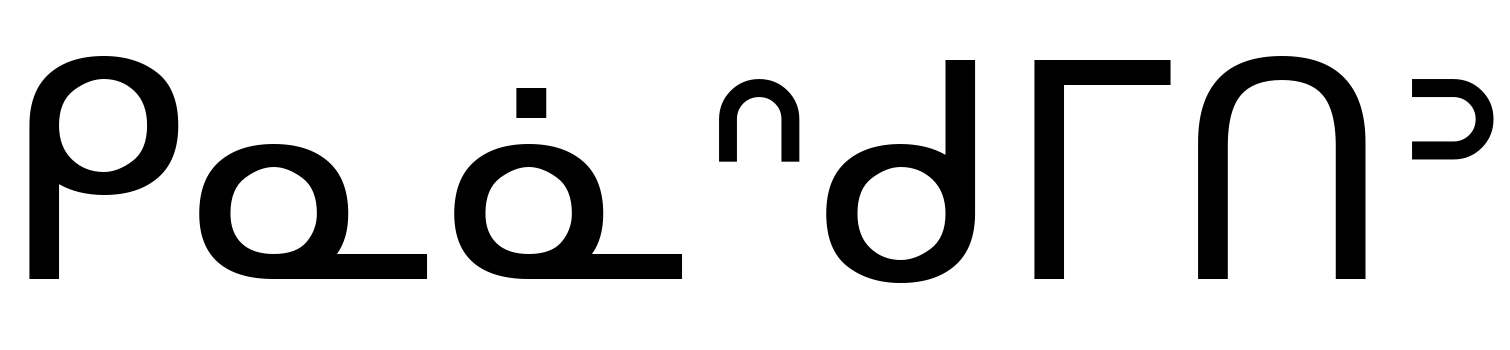
\includegraphics[width=5cm]{kinanaskomitin.png}

  
  
  
\includegraphics[width=6cm]{shukran_lak.png}
\end{center}
  
  
\end{frame}




%%% Local Variables:
%%% TeX-master: "../main.tex"
%%% End:
